% Figure 1: the entry's passes and merge rules, in the style of the team's diagrams/main-diagram.png, with the facts checked
% against src/pipeline.py and Scripts/fleet.py (remask -> override -> countfix). The scene is a synthetic illustration and
% the question is not a VistaQA question; box and mask are drawn over the photo in [0,1] image coordinates. The two logos
% are cut from main-diagram.png. Needs \usetikzlibrary{arrows.meta,shadows.blur}.
\definecolor{aTab}{HTML}{2D68AD}\definecolor{aLine}{HTML}{7DA4E0}\definecolor{aFill}{HTML}{EEF4FD}%
\definecolor{bTab}{HTML}{7E62B0}\definecolor{bLine}{HTML}{B9A1DE}\definecolor{bFill}{HTML}{F5EFFB}%
\definecolor{cTab}{HTML}{D9772F}\definecolor{cLine}{HTML}{EDAA78}\definecolor{cFill}{HTML}{FFF7EE}%
\definecolor{dTab}{HTML}{4A8F35}\definecolor{dLine}{HTML}{98C788}\definecolor{dFill}{HTML}{F3F9EE}%
\definecolor{vlmFill}{HTML}{E6EFFC}\definecolor{vlmLine}{HTML}{7DA4E3}\definecolor{samFill}{HTML}{EFE5FA}\definecolor{samLine}{HTML}{B094DD}%
\definecolor{outFill}{HTML}{EAF5E3}\definecolor{outLine}{HTML}{A6CF93}\definecolor{okg}{HTML}{3E8E24}%
\definecolor{mFill}{HTML}{F8F3FB}\definecolor{mLine}{HTML}{B9A3D9}\definecolor{mNum}{HTML}{8E73BD}\definecolor{oTab}{HTML}{1F4F8F}%
\definecolor{ink}{HTML}{1E1E1E}\definecolor{boxLine}{HTML}{C5CBD4}\definecolor{cardLine}{HTML}{D2D2D8}%
\definecolor{contFill}{HTML}{F7F9FC}\definecolor{contLine}{HTML}{D3DBE8}\definecolor{legFill}{HTML}{F7F7F9}\definecolor{boxred}{HTML}{E34948}%
\def\womanbox{(0.325,0.005) rectangle (0.655,0.675)}%
\def\womanmask{(0.480,0.667) -- (0.536,0.649) -- (0.569,0.589) -- (0.569,0.507) -- (0.559,0.444) -- (0.590,0.422) --
  (0.641,0.360) -- (0.648,0.056) -- (0.574,0.044) -- (0.572,0.005) -- (0.349,0.005) -- (0.331,0.111) -- (0.336,0.211) --
  (0.356,0.356) -- (0.389,0.433) -- (0.402,0.533) -- (0.426,0.633) -- cycle}%
\protected\def\nohy{\hyphenpenalty=10000\relax}%
\newsavebox\scIn\newsavebox\scBox\newsavebox\scBoxB\newsavebox\scMask\newsavebox\scOut%
\newsavebox\icBox\newsavebox\icGear\newsavebox\icCheck\newsavebox\icRefresh%
\newcommand{\scene}[3]{\sbox#1{\begin{tikzpicture}
  \node[anchor=south west, inner sep=0] (im) at (0,0) {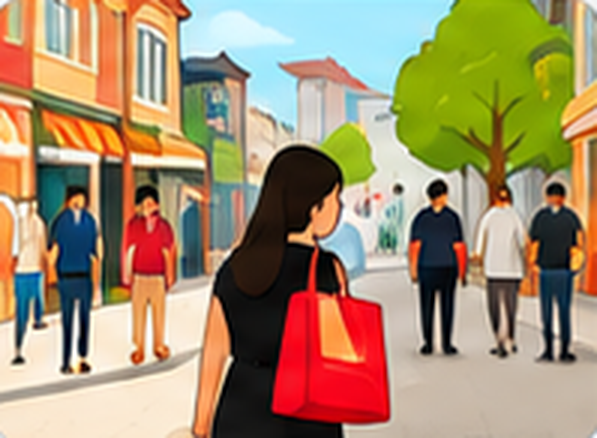
\includegraphics[width=#2]{diagrams/scene.png}};
  \begin{scope}[x={(im.south east)}, y={(im.north west)}] #3 \end{scope}\end{tikzpicture}}}%
\scene\scIn{1.75cm}{}%
\scene\scBox{1.17cm}{\draw[boxred, line width=0.7pt] \womanbox;}%
\scene\scBoxB{0.9cm}{\draw[boxred, line width=0.6pt] \womanbox;}%
\scene\scMask{0.9cm}{\fill[black] (0,0) rectangle (1,1); \fill[white] \womanmask;}%
\scene\scOut{1.55cm}{\fill[black] (0,0) rectangle (1,1); \fill[white] \womanmask;}%
\sbox\icBox{\tikz[baseline=-0.6ex]\draw[rounded corners=0.6pt, line width=0.4pt] (0,-0.065) rectangle (0.13,0.065);}%
\sbox\icGear{\tikz[baseline=-0.6ex]{\foreach \a in {0,45,...,315} \fill[ink, rotate=\a] (-0.026,0.06) rectangle (0.026,0.1);
  \fill[ink] (0,0) circle (0.075); \fill[white] (0,0) circle (0.042); \draw[ink, line width=0.35pt] (0,0) circle (0.022);}}%
\sbox\icCheck{\tikz[baseline=-0.5ex]\draw[white, line width=0.9pt, line cap=round, line join=round] (0,0.01) -- (0.045,-0.04) -- (0.13,0.065);}%
\sbox\icRefresh{\tikz[baseline=-0.6ex]\draw[bTab, line width=0.5pt, -{Stealth[length=0.75mm, width=0.9mm]}] (70:0.07) arc (70:340:0.07);}%
\newcommand\chipt[4]{$\vcenter{\hbox{\includegraphics[height=#2]{diagrams/logo_#1}}}$\hspace{3pt}%
  $\vcenter{\hbox{\def\arraystretch{0.92}\begin{tabular}{@{}l@{}}\textbf{#3}\\#4\end{tabular}}}$}%
%
% rows: A -0.2/-1.42, B -1.57/-2.52, C -2.67/-3.82, D -3.97/-5.36; container 0/-5.45; panels x 2.38..9.27
\begin{tikzpicture}[font=\sffamily\fontsize{6}{7}\selectfont\nohy, line join=round,
  sh/.style={blur shadow={shadow blur steps=6, shadow xshift=0.3pt, shadow yshift=-0.6pt, shadow blur radius=1.4pt, shadow opacity=20}},
  panel/.style 2 args={draw=#1, fill=#2, rounded corners=4pt, line width=0.7pt, sh},
  pill/.style={fill=#1, text=white, font=\sffamily\bfseries\fontsize{6.3}{7}\selectfont, rounded corners=1.6mm,
    inner xsep=4pt, inner ysep=1.5pt, minimum height=0.32cm, anchor=west, sh},
  chip/.style 2 args={draw=#1, fill=#2, rounded corners=3pt, line width=0.55pt, minimum width=1.9cm, minimum height=0.6cm, inner sep=1.5pt, sh},
  vlm/.style={chip={vlmLine}{vlmFill}}, sam/.style={chip={samLine}{samFill}},
  wbox/.style={draw=boxLine, fill=white, rounded corners=3pt, line width=0.45pt, inner sep=2.2pt, align=flush left},
  gbox/.style={draw=outLine, fill=outFill, rounded corners=3pt, line width=0.45pt, inner sep=2.2pt, align=flush left},
  arr/.style={-{Stealth[length=1.5mm, width=1.15mm]}, line width=0.55pt, draw=ink},
  numc/.style={circle, fill=mNum, text=white, font=\sffamily\bfseries\fontsize{5.6}{6}\selectfont, inner sep=0pt, minimum size=0.27cm},
  rule/.style={anchor=north west, text width=1.75cm, inner sep=0, align=flush left},
  leg/.style={anchor=west, inner sep=0, font=\sffamily\fontsize{5.3}{6}\selectfont}]
\useasboundingbox (-0.02,0.05) rectangle (13.95,-5.55);

% ---- input card ----
\draw[fill=white, draw=cardLine, rounded corners=4pt, line width=0.5pt, sh] (0,0) rectangle (1.95,-3.27);
\node[inner sep=0] at (0.975,-0.78) {\usebox\scIn};
\node at (0.975,-1.57) {\itshape Image $\boldsymbol{x}$};
\draw[fill=legFill, draw=cardLine, rounded corners=3pt, line width=0.45pt] (0.1,-1.75) rectangle (1.85,-3.15);
\node[fill=bTab, text=white, rounded corners=1.2pt, inner sep=0pt, minimum size=0.25cm, font=\sffamily\bfseries\fontsize{5.6}{6}\selectfont] at (0.29,-1.95) {Q};
\node[anchor=west, inner sep=0, font=\sffamily\bfseries\fontsize{6.3}{7}\selectfont] at (0.47,-1.95) {Question $\boldsymbol{q}$};
\node[anchor=north west, inner sep=0, text width=1.6cm, align=flush left, font=\sffamily\itshape\fontsize{6}{7}\selectfont\nohy] at (0.17,-2.15) {Which person is carrying a shopping bag?};

% ---- legend card ----
\draw[fill=legFill, draw=cardLine, rounded corners=4pt, line width=0.5pt, sh] (0,-3.42) rectangle (1.95,-5.45);
\node[anchor=west, inner sep=0, font=\sffamily\bfseries\fontsize{6.3}{7}\selectfont] at (0.12,-3.64) {Legend};
\draw[arr] (0.1,-3.92) -- (0.36,-3.92); \node[leg] at (0.43,-3.92) {data flow};
\draw[arr, dashed, draw=bTab] (0.1,-4.22) -- (0.36,-4.22); \node[leg] at (0.43,-4.22) {conditional};
\draw[fill=vlmFill, draw=vlmLine, rounded corners=1.5pt, line width=0.45pt] (0.1,-4.6) rectangle (0.36,-4.44); \node[leg] at (0.43,-4.52) {VLM (Qwen)};
\draw[fill=samFill, draw=samLine, rounded corners=1.5pt, line width=0.45pt] (0.1,-4.9) rectangle (0.36,-4.74); \node[leg] at (0.43,-4.82) {SAM3 segmenter};
\draw[fill=outFill, draw=outLine, rounded corners=1.5pt, line width=0.45pt] (0.1,-5.2) rectangle (0.36,-5.04); \node[leg] at (0.43,-5.12) {Model output};

% ---- container and the four passes ----
\draw[fill=contFill, draw=contLine, rounded corners=5pt, line width=0.5pt, sh] (2.27,0) rectangle (9.38,-5.45);
\draw[panel={aLine}{aFill}] (2.38,-0.2) rectangle (9.27,-1.42);
\draw[panel={bLine}{bFill}] (2.38,-1.57) rectangle (9.27,-2.52);
\draw[panel={cLine}{cFill}] (2.38,-2.67) rectangle (9.27,-3.82);
\draw[panel={dLine}{dFill}] (2.38,-3.97) rectangle (9.27,-5.36);
\node[pill=aTab] at (2.48,-0.2) {A. Answer and evidence boxes};
\node[pill=bTab] at (2.48,-1.57) {B. Masks from boxes};
\node[pill=cTab] at (2.48,-2.67) {C. Premise check (answer-agnostic)};
\node[pill=dTab] at (2.48,-3.97) {D. Counters (plain counting questions)};

% bus from the input to every pass; D runs only on counting questions
\draw[line width=0.55pt, draw=ink] (1.95,-2.45) -- (2.12,-2.45);
\draw[line width=0.55pt, draw=ink] (2.12,-0.7) -- (2.12,-3.28);
\foreach \y in {-0.7,-2.1,-3.28} \draw[arr] (2.12,\y) -- (2.38,\y);
\draw[arr, dashed, draw=dTab] (2.12,-3.28) -- (2.12,-4.75) -- (2.38,-4.75);

% A
\node[vlm] (a) at (3.45,-0.68) {\chipt{qwen}{0.3cm}{Qwen3.6-27B}{(NF4, 4-bit)}};
\node[draw=bTab, dashed, fill=bFill, rounded corners=1.4mm, line width=0.5pt, inner xsep=2.5pt, inner ysep=1.2pt,
  font=\sffamily\fontsize{5.2}{6}\selectfont] (rw) at (3.5,-1.18) {\usebox\icRefresh\hspace{2pt}\textbf{Rewrite} if $\leq$3 words};
\node[wbox, text width=2.95cm] (aout) at (6.2,-0.86) {\textbf{Answer:} \emph{The woman in front is carrying a red bag.}\\[1pt]
  \textbf{Boxes:} \usebox\icBox\ $[x_1, y_1, x_2, y_2]$ \dots};
\node[inner sep=0] (athumb) at (8.565,-0.86) {\usebox\scBox};
\draw[arr] (a.east) -- (a.east -| aout.west);
\draw[arr] (aout) -- (athumb);

% B
\node[sam] (b) at (3.45,-2.1) {\chipt{sam3}{0.24cm}{SAM3}{(box prompts)}};
\node[inner sep=0] (bbox) at (5.42,-2.1) {\usebox\scBoxB};
\node[inner sep=0] (bmask) at (6.57,-2.1) {\usebox\scMask};
\node[wbox, text width=1.8cm, align=center] (bout) at (8.21,-2.1) {One mask per box\\(full resolution)};
\draw[arr] (b) -- (bbox); \draw[arr] (bbox) -- (bmask); \draw[arr] (bmask) -- (bout);
\draw[arr, draw=bTab] (aout.south -| bbox) -- (bbox.north);

% C
\node[vlm] (c) at (3.45,-3.28) {\chipt{qwen}{0.3cm}{Qwen3-VL-8B}{(fp16)}};
\node[wbox, text width=3.0cm, font=\sffamily\fontsize{5.5}{6.4}\selectfont\nohy] (cout) at (6.22,-3.31) {\textbf{Task:} Name any \emph{X} the
  question assumes but the image lacks, then ask: \emph{Is there any X in the image?}};
\node[gbox, align=center, text width=0.95cm] (cres) at (8.62,-3.31) {\textbf{Missing:}\\\textcolor{okg}{\textbf{none}}};
\draw[arr] (c) -- (cout); \draw[arr] (cout) -- (cres);

% D
\node[sam, inner ysep=0.8pt] (d1) at (3.45,-4.44) {\chipt{sam3}{0.24cm}{SAM3}{(text prompt)}};
\node[vlm, inner ysep=0.8pt] (d2) at (3.45,-5.04) {\chipt{qwen}{0.3cm}{Qwen3-VL-8B}{(fp16)}};
\node[gbox, text width=1.8cm] (g1) at (5.72,-4.44) {\textbf{Label} from \textbf{A}\\(score $\geq$ 0.8)};
\node[gbox, text width=1.8cm] (g2) at (5.72,-5.04) {\textbf{Count from VLM}};
\node[draw=ink, fill=white, rounded corners=2.5pt, line width=0.55pt, inner sep=2pt] (mx) at (7.42,-4.74) {max};
\node[gbox, text width=1.05cm] (g3) at (8.62,-4.74) {\textbf{Counter:} only raises A's count};
\draw[arr] (d1) -- (g1); \draw[arr] (d2) -- (g2);
\draw[arr, rounded corners=2pt] (g1.east) -- ++(0.17,0) |- ([yshift=1.2pt]mx.west);
\draw[arr, rounded corners=2pt] (g2.east) -- ++(0.17,0) |- ([yshift=-1.2pt]mx.west);
\draw[arr] (mx) -- (g3);

% ---- rule-based merge ----
\draw[panel={mLine}{mFill}] (9.62,-0.6) rectangle (11.88,-4.85);
\begin{scope}\clip[rounded corners=4pt] (9.62,-0.6) rectangle (11.88,-4.85); \fill[white] (9.62,-0.6) rectangle (11.88,-1.05); \end{scope}
\draw[mLine, line width=0.7pt, rounded corners=4pt] (9.62,-0.6) rectangle (11.88,-4.85);
\draw[mLine, line width=0.4pt] (9.62,-1.05) -- (11.88,-1.05);
\node[anchor=west, inner sep=0, font=\sffamily\bfseries\fontsize{6}{7}\selectfont] at (9.72,-0.825) {\usebox\icGear\hspace{3pt}Rule-based Merge};
\node[numc] at (9.84,-1.3) {1}; \node[rule] at (10.03,-1.2) {Attach \textbf{B}'s masks to \textbf{A}'s answer, one per box.};
\draw[mLine, line width=0.35pt] (9.75,-2.0) -- (11.75,-2.0);
\node[numc] at (9.84,-2.25) {2}; \node[rule] at (10.03,-2.15) {If \textbf{C} names \emph{X} and \emph{Is there any X?} gets
  \textbf{no}: answer = ``There is no X in the image.'', masks~=~$\emptyset$.};
\draw[mLine, line width=0.35pt] (9.75,-3.62) -- (11.75,-3.62);
\node[numc] at (9.84,-3.87) {3}; \node[rule] at (10.03,-3.77) {If a plain counting question: raise \textbf{A}'s count to the
  larger counter from \textbf{D}.};
\draw[arr, draw=aTab, rounded corners=2pt] (9.27,-0.86) -- (9.47,-0.86) |- (9.62,-1.38);
\draw[arr, draw=bTab, rounded corners=2pt] (9.27,-2.1) -- (9.52,-2.1) |- (9.62,-1.62);
\draw[arr, draw=cTab] (9.27,-3.0) -- (9.62,-3.0);
\draw[arr, draw=dTab, rounded corners=2pt] (9.27,-4.75) -- (9.47,-4.75) |- (9.62,-4.15);

% ---- final output ----
\draw[arr] (11.88,-2.5) -- (12.1,-2.5);
\draw[draw=oTab, fill=white, rounded corners=4pt, line width=0.8pt, sh] (12.1,-0.85) rectangle (13.92,-4.1);
\node[pill=oTab, anchor=center, minimum width=1.68cm] at (13.01,-0.85) {\usebox\icCheck\hspace{3pt}Final Output};
\node[anchor=west, inner sep=0, font=\sffamily\bfseries\fontsize{6.3}{7}\selectfont] at (12.2,-1.25) {Answer:};
\node[gbox, text width=1.5cm, font=\sffamily\itshape\fontsize{6}{7}\selectfont\nohy] at (13.01,-2.0) {The woman in front is carrying a red bag.};
\node[anchor=west, inner sep=0, font=\sffamily\bfseries\fontsize{6.3}{7}\selectfont] at (12.2,-2.72) {Masks:};
\node[inner sep=0] at (13.01,-3.42) {\usebox\scOut};
\end{tikzpicture}%
